\chapter{Implementazione}
\label{cap:implementazione}

L'implementazione del PoC è una parte fondamentale del progetto di stage, in quanto permette di verificare la fattibilità del prodotto e di valutare la bontà delle scelte progettuali.\\
In questo capitolo verranno descritte le principali scelte implementative, sia per quanto riguarda il frontend che il backend.\\

\section{Struttura del progetto}
La struttura del progetto è stata organizzata in modo da separare il frontend dal backend, in modo da poterli sviluppare in modo indipendente. Inoltre, è stato scelto di utilizzare una repository su Azure DevOps per il versioning del codice, in modo da poter avere una storicizzazione delle modifiche.
\section{Backend}
Il backend è stato sviluppato utilizzando il linguaggio di programmazione C\texttt{\#} e il framework ASP.NET Core, è basato sul template fornito dall'azienda che prevede l'utilizzo di un'architettura a layer.\\
Come ambiente di sviluppo è stato utilizzato Visual Studio 2022.\\
\subsection{Architettura a layer}
L'architettura a layer è una tipologia di architettura software che prevede la suddivisione del codice in diversi livelli, ognuno dei quali ha un compito ben preciso, e che comunica con gli altri livelli attraverso interfacce. Questo permette di avere un codice più modulare e mantenibile, in quanto ogni livello ha un compito ben preciso e non si occupa di altro.\\
Il backend è composto da un unico progetto "AdMaioraStreamingPOC", che contiene i vari layer suddivisi in cartelle, ognuna delle quali contiene le soluzioni relative al layer. I layer sono: API, Core e Data.\\

\subsubsection{API}
Il layer API è il livello più esterno dell'applicazione, si occupa di gestire le richieste HTTP in arrivo dal frontend. È divisa in due soluzioni: Controller e DTO.\\
\begin{itemize}
    \item \textbf{Controllers}: sono le classi che si occupano di gestire le richieste HTTP in arrivo dal frontend, utilizzano il framework ASP.NET Core e la libreria AutoMapper per la conversione dei DTO in entità e viceversa; inoltre, utilizzano la dependency injection per iniettare le dipendenze necessarie dalle classi di Service presenti nel layer Core, l'uso di questa tecnica rende i controller indipendenti dalle implementazioni concrete delle dipendenze.\\
    Per ogni entità del database è stato creato un controller, che contiene metodi CRUD e non, per gestire le richieste HTTP in modo completo. Quando un controller riceve una richiesta HTTP, utilizza i metodi presenti nel Service per gestire la richiesta, e restituisce al frontend il risultato della richiesta in formato JSON.\\
    \item \textbf{DTO}: sono classi che contengono la struttura dei dati che vengono scambiati tra il frontend e il backend.
    Per ogni entità del database sono stati creati tre DTO: uno per la creazione, uno per l'aggiornamento e uno per la visualizzazione; così facendo, si evita di scambiare dati inutili tra frontend e backend, e si evita di dover gestire la serializzazione e deserializzazione di dati inutili. Inoltre, utilizzando i DTO, si evita di dover esporre le entità del database al frontend, favorendo la separazione tra frontend e backend.\\
\end{itemize}
\subsubsection{Core}
Il layer Core è il livello intermedio dell'applicazione, e si occupa di gestire la logica di business dell'applicazione. È diviso in due soluzioni: Model e Services.\\
\begin{itemize}
    \item \textbf{Model}: sono classi che rappresentano le entità nel database, il loro scopo è quello di mappare le entità del database in classi C\texttt{\#}, in modo da poterle utilizzare all'interno della logica del codice. Per ogni entità del database è stato creato un Model, che contiene le proprietà dell'entità.\\
    \item \textbf{Services}: sono classi che si occupano di gestire la logica di business dell'applicazione, utilizzano i Model per accedere ai dati nel database, e li restituiscono al layer API. Per ogni entità del database è stato creato un Service, che contiene  metodi CRUD e non, per gestire la logica di business dell'applicazione. Fornisce i metodi al layer API attraverso interfacce, inoltre vengono iniettate le dipendenze necessarie del Provider presente nel layer Data, le credenziali per l'accesso ad Azure e della configurazione per il server TUS.io. Il suo scopo principale è quello di fornire un'interfaccia tra il layer API e il layer Data. Inoltre si occupa anche della comunicazione con i servizi esterni, infatti gestisce l'upload dei video su Azure Media Services, tramite le sue API dedicate e comunica con l'istanza TUS.io.\\
\end{itemize}
\subsubsection{Data}
Il layer Data è il livello più interno dell'applicazione, e si occupa di gestire l'accesso ai dati nel database. È diviso in tre soluzioni: Context, Providers e Entity.\\
\begin{itemize}
\item \textbf{Context}: è la classe che si occupa di gestire l'accesso ai dati nel database, che quando viene inizializzato, gli viene iniettata la configurazione per il collegamento e definisce tre proprietà di tipo DbSet, una per ogni entità del database, che consentono di effettuare operazione di query e manipolazione dei dati.\\
\item \textbf{Providers}: sono classi che si occupano di gestire l'accesso ai dati nel database, utilizzando il Context per accedervi, e li restituiscono al layer Core convertendoli in Model tramite AutoMapper. È stata creata una classe per ogni entità del database, e contengono i metodi CRUD per gestire l'accesso ai dati nel database. Lo scopo principale dei providers è quindi quello di fornire un'interfaccia tra il layer Core e il database.\\
\item \textbf{Entity}: sono classi che rappresentano le entità nel database, il loro scopo è quello di mappare le entità del database in classi C\texttt{\#}, in modo da poterle utilizzare all'interno della logica del codice. Per ogni entità del database è stato creato un Entity, che contiene le proprietà dell'entità. Queste classi sono utilizzate dal Context per accedere ai dati nel database. Oltre a ciò, vengono utilizzate per definire le proprietà, tramite il framework Entity Framework Core e il suo sistema di migrazioni: quando viene modificata una proprietà di un Entity, viene eseguita una migrazione che modifica la struttura del database in base alle modifiche apportate.\\
\end{itemize}
\section{Frontend}
Il frontend è stato sviluppato utilizzando il framework React e la libreria grafica Material-UI.\\
Il frontend è diviso in tre cartelle principali: Components, Pages e Services, utilizzando il template fornito dall'azienda che prevede l'utilizzo del template Container-Presenter.\\
È stato utilizzato Visual Studio code come ambiente di sviluppo, e Node.js come runtime per l'esecuzione del codice.\\

\subsection{Architettura}
L'architettura del frontend è divisa in tre cartelle: Pages, Common e Context.

\subsubsection{Pages}
La cartella Pages contiene le pagine dell'applicazione, ovvero le pagine che vengono visualizzate dall'utente. Ogni pagina è divisa a sua volta in tre componenti: Context, Page e Components.\\

\begin{itemize}
    \item \textbf{Context}: svolge il ruolo di fornire un meccanismo per l'accesso e la condivisione dei dati tra i componenti, in modo da evitare di dover passare i dati da un componente all'altro. Per ogni pagina è stato creato un Context, che contiene un provider che contiene lo stato e le funzioni per l'accesso ai dati; ogni componente avvolto dal provider può accedere ai dati e alle funzioni per modificarli. L'accesso ai dati avviene tramite l'utilizzo del context di FetchContext, che contiene le route per effettuare le chiamate al backend.\\
    \item \textbf{Page}: Ogni pagina contiene un componente PageContent, che renderizza i componenti della pagina. Successivamente essi vengono avvolti dal Provider della pagina specifica che permette l'accesso al Context della pagina, in modo tale che possano accedere ai dati e alle funzioni per modificarli.\\
    \item \textbf{Components}: sono le porzioni di codice che vengono renderizzate all'interno della pagina.
\end{itemize}
\subsubsection{Common}
La cartella Common contiene i componenti che vengono utilizzati in tutte le pagine, è composto da tre file:
\begin{itemize}
    \item \textbf{Layout}:definisce la struttura di ogni pagina, composta a sinistra da un menù laterale, sopra dal titolo della pagina corrente e al centro dal contenuto della pagina passato come props.
    Il menù laterale è composto da una lista di MenuItems, che vengono renderizzati grazie all'utilizzo del context di NavContext.
    \item \textbf{Route}: permette di navigare tra le pagine in base al percorso specificato contenuto nel MenuItems.\\
    \item \textbf{DialogCustom}: è un componente che permette di visualizzare un dialog, che contiene un titolo, un contenuto e due bottoni, uno per confermare e uno per annullare. Viene utilizzato in tutte le pagine per confermare le azioni che possono modificare i dati nel database. Il contenuto viene passato tramite props, in modo da poterlo personalizzare in base alla pagina. L'utilizzo di questo componente permette di evitare di dover creare un dialog pressoché identico in tutte le pagine.\\
\end{itemize}
\subsubsection{Context}
La cartella Context, contiene i file di contesto, è composta da tre file: FetchContext, NavContext e ToastContext.
\begin{itemize}
    \item \textbf{FetchContext}: contiene le route per effettuare le chiamate al backend, è composto da una funzione "Compile Route" che permette di comporre la route in base ai parametri passati, e da una funzione "Fetch" che permette di effettuare la chiamata al backend. Questo permette di evitare di dover ripetere le route in ogni componente.\\
    \item \textbf{NavContext}: contiene le route per effettuare la navigazione tra le pagine, è composto da vari metodi per per la navigazione, per la gestione del menù laterale, per la gestione del titolo della pagina e per la gestione del breadcrumb. \\
    \item \textbf{ToastContext}: contiene le funzioni per mostrare i toast, composto da quattro funzioni: "Success", "Error", "Warning" e "Info", che permettono di mostrare un toast con il messaggio passato come parametro.\\
\end{itemize}
\subsection{Interfaccia grafica}
\subsubsection{Pagina Home}
La pagina Home è la pagina principale dell'applicazione, contiene una grid di tutti gli eventi disponibili, e un menù laterale che permette la navigazione tra le pagine.\\
In figura \ref{fig:home} è rappresentano un esempio della pagina home sviluppata.
\begin{figure}[H]
    \centering
    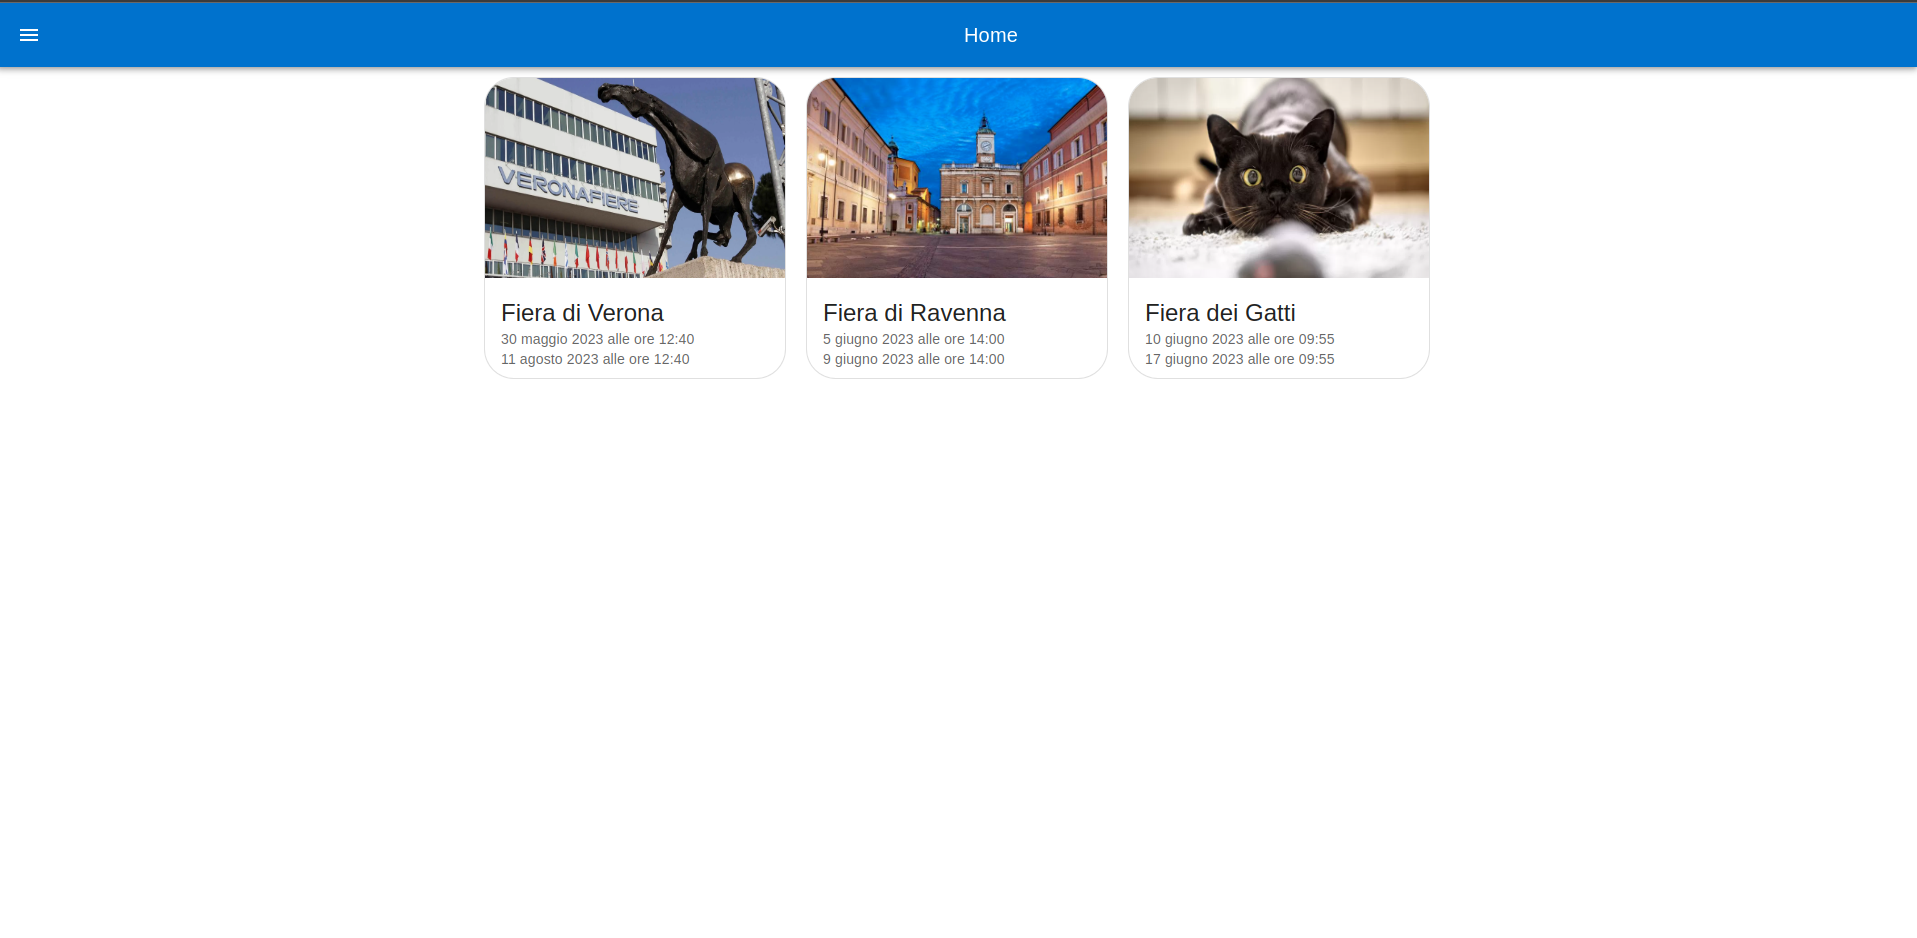
\includegraphics[width=1\textwidth]{images/interface/home.png}
    \caption{Pagina Home}
    \label{fig:home}
\end{figure}
\subsubsection{Pagina Eventi}
Quando si clicca su un evento nella pagina Home, si viene reindirizzati alla pagina dell'evento, che contiene una grid con tutti i video dell'evento.\\
In figura \ref{fig:eventi} è rappresentano un esempio della pagina di un evento inserito nel sistema.
\begin{figure}[H]
    \centering
    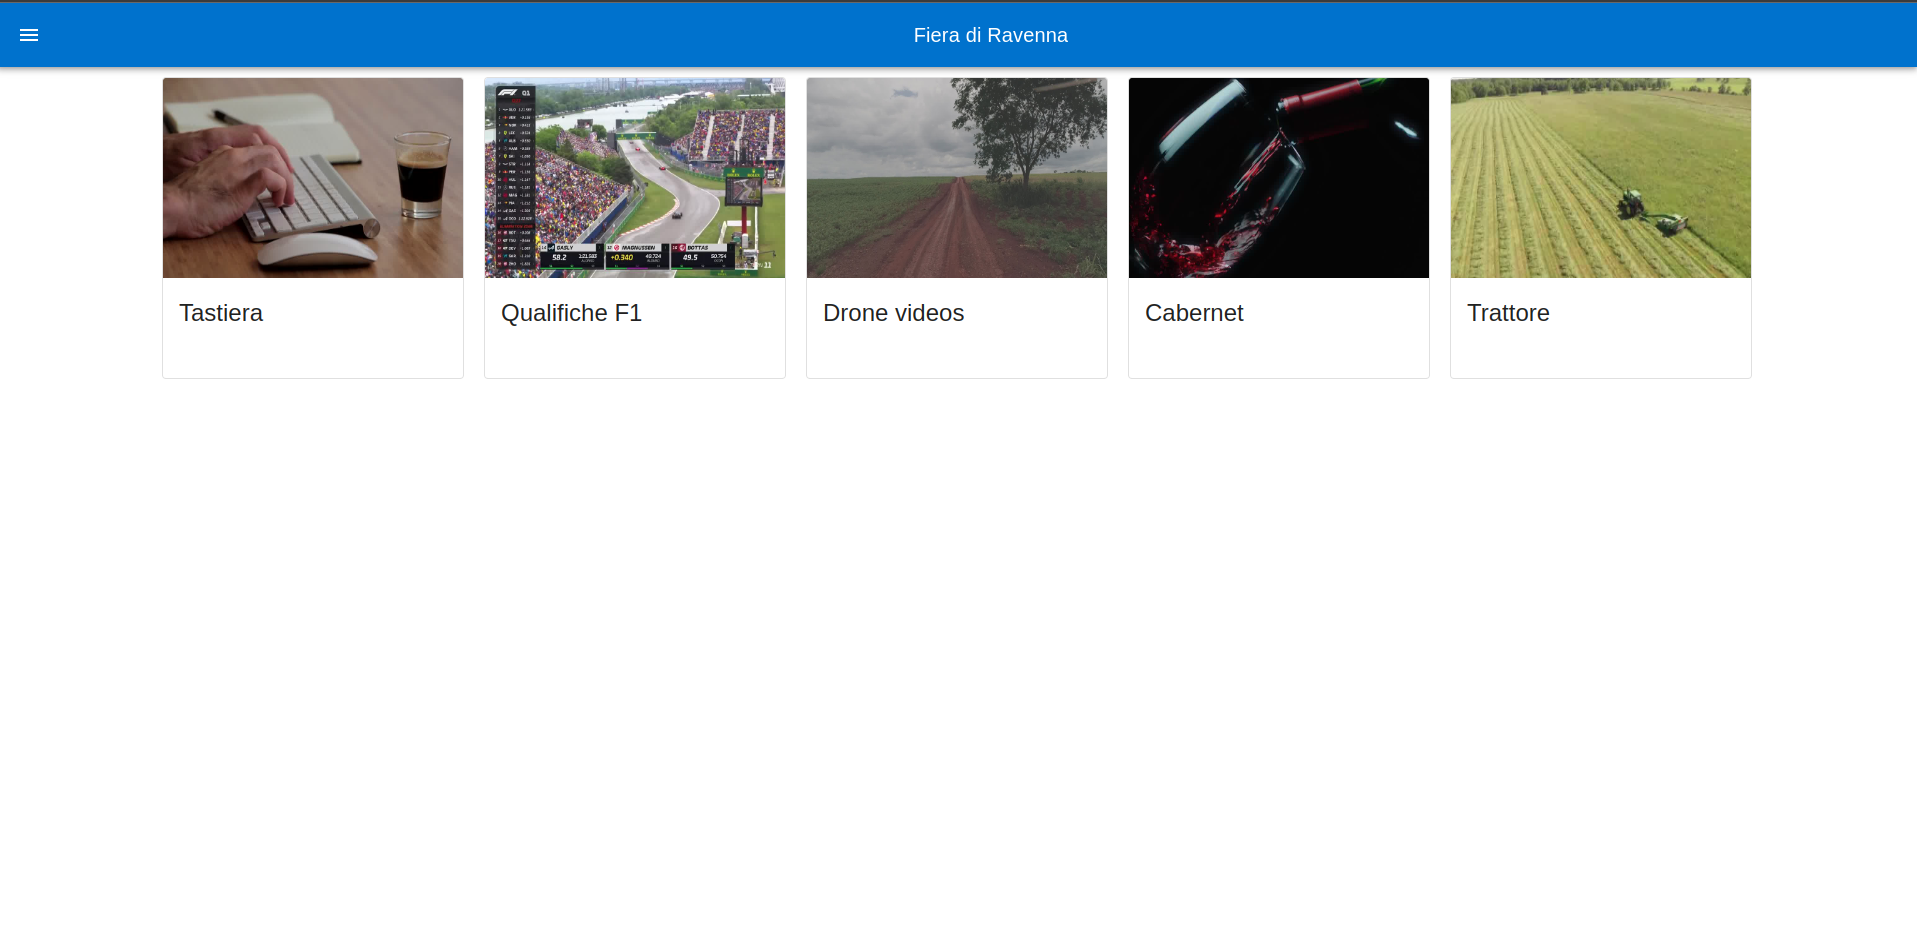
\includegraphics[width=1\textwidth]{images/interface/events.png}
    \caption{Pagina Eventi}
    \label{fig:eventi}
\end{figure}
\subsubsection{Pagina Video}
Quando si clicca su un video nella pagina Eventi, si viene reindirizzati alla pagina del video, che contiene il player del video e i pulsanti per la gestione.\\
In figura \ref{fig:video} è rappresentano un esempio di visualizzazione di un video.
\begin{figure}[H]
    \centering
    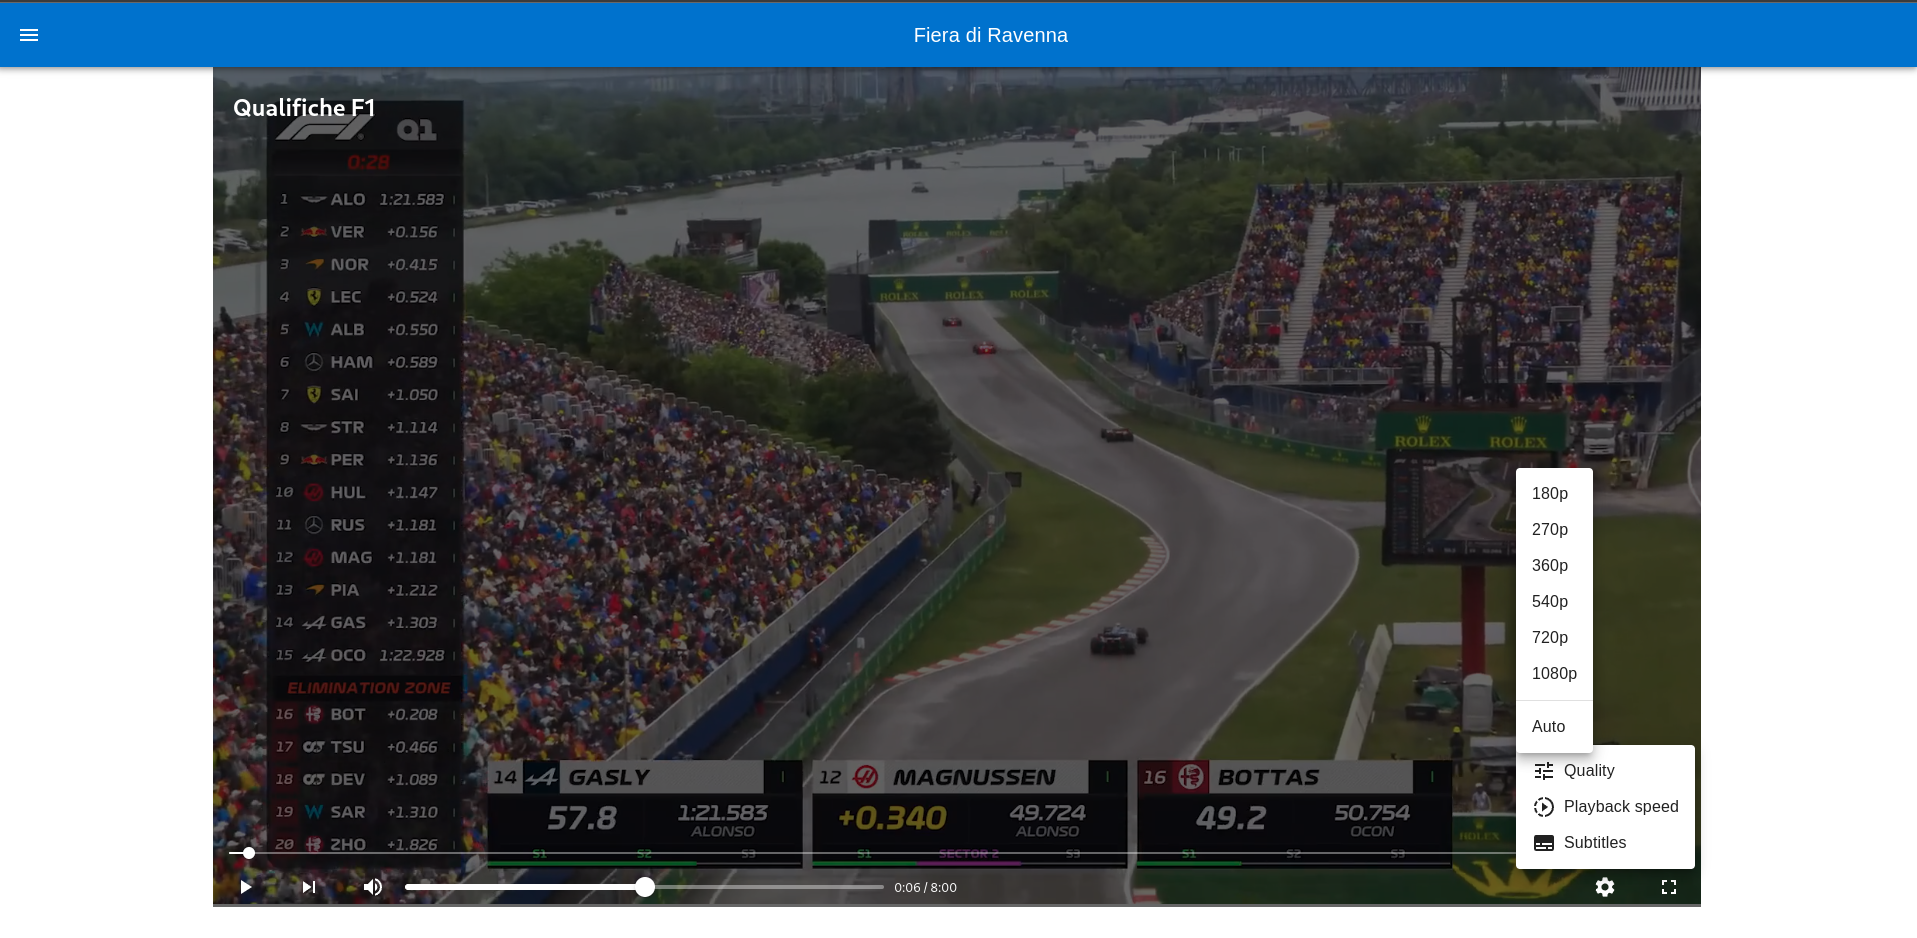
\includegraphics[width=1\textwidth]{images/interface/video.png}
    \caption{Pagina Video}
    \label{fig:video}
\end{figure}
\subsubsection{Pagina Gestione}
Le pagine di gestione sono tre, una per gli eventi, una per i video e una per gli utenti. Ogni pagina contiene una tabella con tutti gli elementi, ogni riga contiene due pulsanti, uno per modificare l'elemento e uno per eliminarlo. Inoltre è presente anche un pulsante per aggiungere un nuovo elemento attraverso un dialog.\\
In figura \ref{fig:gestionevideo} è rappresentana la pagina della tabella per la gestione dei video.
\begin{figure}[H]
    \centering
    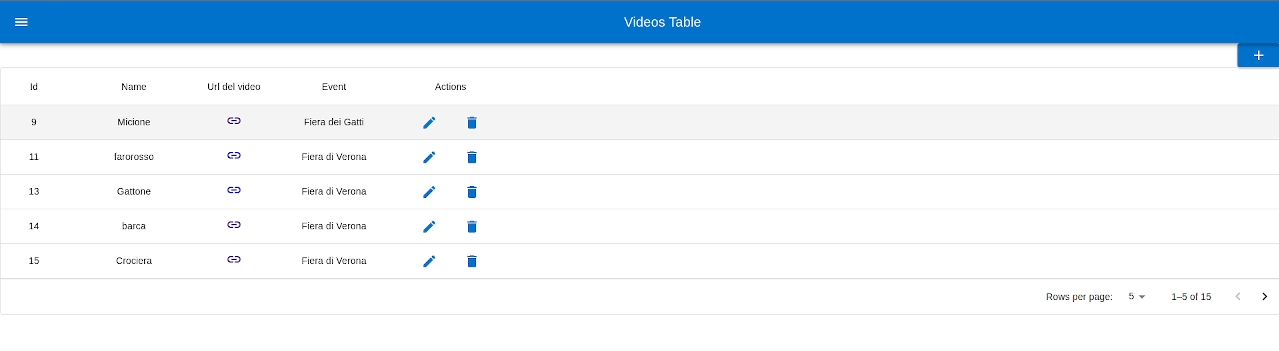
\includegraphics[width=1\textwidth]{images/interface/videotable.png}
    \caption{Pagina Gestione dei video}
    \label{fig:gestionevideo}
\end{figure}
Quando viene premuta l'icona della matita, si apre un dialog, come in figura \ref{fig:modifica video}, tramite la quale l'utente può modificare i dati del video.
\begin{figure}[H]
    \centering
    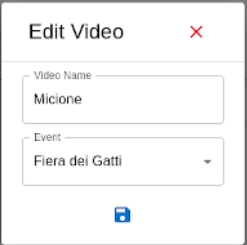
\includegraphics[width=0.3\textwidth]{images/interface/editvideo.png}
    \caption{Dialog Modifica Video}
    \label{fig:modifica video}
\end{figure}
Quando viene premuto il bottone di aggiunta, si apre un dialog, come in figura \ref{fig:aggiuntavideo}, tramite il quale l'utente può selezionare un video da caricare e i dati relativi ad esso.
\begin{figure}[H]
    \centering
    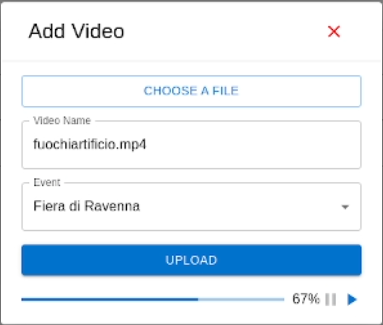
\includegraphics[width=0.3\textwidth]{images/interface/addvideo.png}
    \caption{Dialog Aggiunta Video}
    \label{fig:aggiuntavideo}
\end{figure}
\section{Integrazione con Azure}
Per l'integrazione con i servizi di Azure, sono state utilizzate le API ufficiali fornite da Microsoft, che permettono di gestire i servizi di Azure in modo semplice e veloce.\\
La connessione al database è stata gestita mediante l'utilizzo del framework Entity Framework Core; quando il programma viene inizializzato, nel backend al livello del provider viene iniettata la configurazione per il collegamento al database, che contiene le credenziali per l'accesso al database. Per quanto riguarda il collegamento con Azure Media Service, e vengono utilizzate nel backend nel layer Service per comunicare con le API proprietarie.

\section{Integrazione con TUS.io}
Per la gestione dell'upload dei video dal frontend al backend, è stato utilizzato il servizio TUS.io, che permette di gestire l'upload di file di grandi dimensioni e di gestirne lo stato. Quando viene inizializzato il programma, viene creata un'istanza del server TUS.io, che permette al frontend tramite le API di accedere ad esso e di gestire l'upload dei file. Quando un file viene caricato sul server TUS.io, il frontend invia una chiamata al backend con l'id TUS del file caricato e poi viene passato ai metodi del Service, che si occupa di recuperare il file e successivamente di caricarlo su Azure Media Services.\\
